% Orbital rendezvous RL — 30-minute interview deck (≈10 min talk + appendix for Q&A)
% Build: cd interview_deck && tectonic deck.tex
\documentclass[aspectratio=169,11pt]{beamer}
\usepackage{amsmath,amssymb,booktabs,tikz,graphicx,multicol}
\usetikzlibrary{arrows.meta,positioning,calc,shapes.geometric,fit,backgrounds}
\usepackage{pgfplots}\pgfplotsset{compat=1.18}
\graphicspath{{figs/}}

% ---------- theme ----------
\usetheme{default}
\usecolortheme{seagull}
\definecolor{navy}{HTML}{1F3A5F}
\definecolor{accent}{HTML}{D7301F}
\definecolor{blue2}{HTML}{2C7FB8}
\definecolor{amber}{HTML}{F0A202}
\definecolor{earth}{HTML}{9ECAE1}
\definecolor{grey}{HTML}{666666}
\setbeamercolor{structure}{fg=navy}
\setbeamercolor{title}{fg=navy}
\setbeamercolor{frametitle}{fg=navy,bg=white}
\setbeamercolor{block title}{fg=white,bg=navy}
\setbeamercolor{block body}{bg=navy!6}
\setbeamerfont{frametitle}{series=\bfseries,size=\large}
\setbeamertemplate{navigation symbols}{}
\setbeamertemplate{footline}{%
  \hfill\scriptsize\textcolor{grey}{\insertframenumber}\hspace{3mm}\vspace{2mm}}
\setbeamertemplate{itemize items}[circle]
\setbeamertemplate{section in toc}[sections numbered]
\newcommand{\key}[1]{\textcolor{accent}{\textbf{#1}}}
\newcommand{\src}[1]{\\[1mm]{\tiny\textcolor{grey}{#1}}}
\newcommand{\dv}{\ensuremath{\Delta v}}

% ---------- headline numbers (edit here, not on slides) ----------
\newcommand{\nObs}{38}
\newcommand{\nParams}{139{,}281}
\newcommand{\nEnvs}{1024}
\newcommand{\boxR}{30\,km}
\newcommand{\boxV}{50\,m/s}
\newcommand{\tightR}{5\,km}
\newcommand{\tightV}{1\,m/s}
\newcommand{\headlineSeeds}{5/5 training seeds}
\newcommand{\stepRate}{\(\sim\)740\,k}
\newcommand{\lambertRatio}{1.18\(\times\)}
\newcommand{\boxRatio}{1.55\(\times\)}
\newcommand{\hohmannRatio}{2.38\(\times\)}
\newcommand{\pNinetyNine}{62\,\(\mu\)s}

\title{Learning Orbital Rendezvous}
\subtitle{A reinforcement-learned guidance policy, closed through a bearings-only navigation filter}
\author{Peter Brown}
\date{October 2026}

\begin{document}

% =====================================================================
\begin{frame}[plain]
  \titlepage
  \begin{center}\small\textcolor{grey}{
  One policy; seven rendezvous skills in 3-D with J2; 96--99.5\% held-out success on the five wide-box skills.\\
  Everything shown was measured on held-out episodes under corrected dynamics.}
  \end{center}
  \note{Claim in one line: I built a flight-like GNC loop (simulator, angles-only sensor, filter, learned guidance) in C and PyTorch and verified it the way a certification reviewer would. 10 minutes, then questions.}
\end{frame}

% =====================================================================
\begin{frame}{The problem: get a chaser into a box around a non-maneuvering target}
\begin{columns}[T]
\begin{column}{0.46\textwidth}
\centering
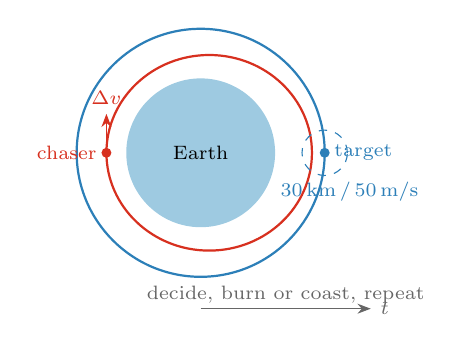
\begin{tikzpicture}[scale=0.9]
  \fill[earth] (0,0) circle (1.05);
  \node[font=\scriptsize] at (0,0) {Earth};
  \draw[blue2,thick] (0,0) circle (1.75);
  \draw[accent,thick] (0.12,0) ellipse (1.45 and 1.38);
  \fill[accent] (-1.33,0) circle (0.07) node[left,font=\scriptsize,accent] {chaser};
  \fill[blue2] (1.75,0) circle (0.07) node[right,font=\scriptsize,blue2] {target};
  \draw[blue2,dashed] (1.75,0) circle (0.32);
  \node[font=\scriptsize,blue2] at (2.1,-0.55) {\boxR\,/\,\boxV};
  \draw[-{Stealth},accent] (-1.33,0) -- ++(0,0.55) node[above,font=\scriptsize] {\dv};
  \draw[grey,-{Stealth}] (0,-2.2) -- (2.4,-2.2) node[right,font=\scriptsize] {$t$};
  \node[font=\scriptsize,grey] at (1.2,-2.0) {decide, burn or coast, repeat};
\end{tikzpicture}
\end{column}
\begin{column}{0.54\textwidth}
\small
\textbf{Success} \; $|\mathbf r_c-\mathbf r_t| < \boxR$ and $|\mathbf v_c-\mathbf v_t| < \boxV$\\[1mm]
\textbf{Failure, any of} \; re-entry \;$\cdot$\; escape ($E\ge 0$) \;$\cdot$\; tank empty \;$\cdot$\; clock expires\\[2mm]
\textbf{Budgets} \; 478\,m/s of \dv\ (15\,\% propellant, Isp 300\,s, Tsiolkovsky), about 2.2$\times$ a Hohmann transfer across the band; a wall clock counted in 60\,s sub-steps\\[2mm]
\textbf{Start} \; random LEO orbits, any phase gap up to $\pm180^\circ$, independent eccentricity and apse orientation\\[2mm]
\textbf{Agent sees} \; \nObs\ floats: its own elements, fuel, the \emph{estimated} target, a target-centred relative-motion block, the clock\\[2mm]
\textbf{Agent does} \; one of 31 discrete actions: an impulsive burn, or a coast of 1\,min to 24\,h
\end{column}
\end{columns}
\note{Two spacecraft; target is passive. The box is a far-field rendezvous criterion (30 km, 50 m/s); the tight-box skill uses 5 km / 1 m/s. No per-step time limit; episodes end for physical reasons or a clock. Fuel 478 m/s versus 217 m/s for a textbook Hohmann 400->800 km (2.2x), so the agent cannot brute-force.}
\end{frame}

% =====================================================================
\begin{frame}{The loop: this is a GNC stack, not a reward-hacking toy}
\centering
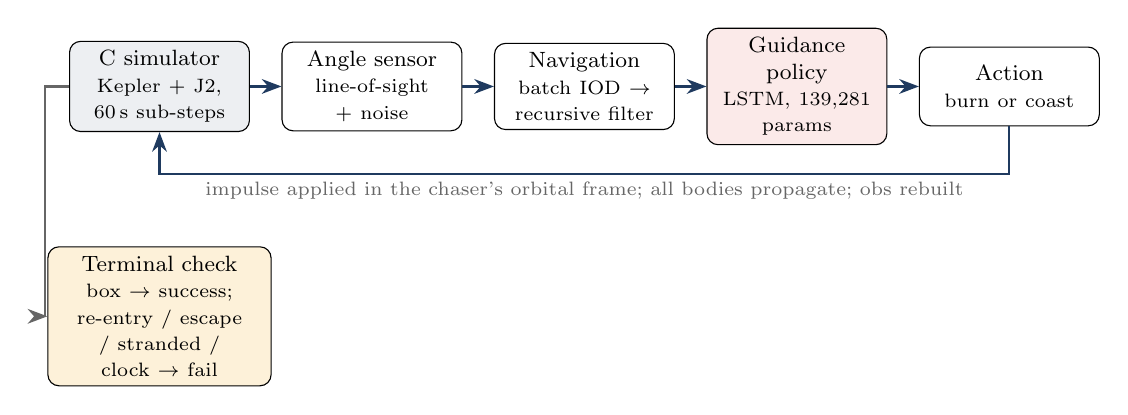
\begin{tikzpicture}[
  box/.style={draw,rounded corners,minimum height=1.0cm,text width=2.05cm,align=center,font=\footnotesize,fill=white},
  arr/.style={-{Stealth[length=2.5mm]},thick,navy}]
  \node[box,fill=navy!8] (sim) {C simulator\\{\scriptsize Kepler + J2, 60\,s sub-steps}};
  \node[box,right=0.4cm of sim] (sen) {Angle sensor\\{\scriptsize line-of-sight + noise}};
  \node[box,right=0.4cm of sen] (nav) {Navigation\\{\scriptsize batch IOD $\to$ recursive filter}};
  \node[box,right=0.4cm of nav,fill=accent!10] (pol) {Guidance policy\\{\scriptsize LSTM, \nParams\ params}};
  \node[box,right=0.4cm of pol] (act) {Action\\{\scriptsize burn or coast}};
  \draw[arr] (sim) -- (sen); \draw[arr] (sen) -- (nav); \draw[arr] (nav) -- (pol); \draw[arr] (pol) -- (act);
  \draw[arr] (act.south) |- ++(0,-0.6) -| (sim.south);
  \node[font=\scriptsize,grey] at ($(sim.south)!0.5!(act.south)+(0,-0.78)$) {impulse applied in the chaser's orbital frame; all bodies propagate; obs rebuilt};
  \node[box,below=1.45cm of sim,text width=2.6cm,fill=amber!15] (gate) {Terminal check\\{\scriptsize box $\to$ success; re-entry / escape / stranded / clock $\to$ fail}};
  \draw[arr,grey] (sim.west) -- ++(-0.3,0) |- (gate.west);
\end{tikzpicture}
\vspace{2mm}
\begin{itemize}\small
  \item Guidance never sees truth in the bearings-only configuration; it flies on the filter's estimate.
  \item The same loop runs in allocation-free C99 on the embedded-style port: bounded execution, action stream identical to PyTorch over 200 episodes.
\end{itemize}
\note{Walk left to right. This mirrors the whiteboard architecture row. Emphasise the policy only sees the estimate. For Huber: an EO sensor gives you exactly these angles; the nav block is the part his payloads feed.}
\end{frame}

% =====================================================================
\begin{frame}{Simulator: analytic two-body plus J2, written in C}
\begin{columns}[T]
\begin{column}{0.55\textwidth}\footnotesize
\textbf{State} \; $(a, e, i, \Omega, \omega, M)$ per body; Cartesian when needed\\[1.5mm]
\textbf{Propagation} \; $M \mathrel{+}= n\,\Delta t$, then Kepler's equation by Newton--Raphson
\[ f(E)=E-e\sin E-M,\qquad E \leftarrow E-\frac{f}{1-e\cos E} \]
true anomaly from $\tan\frac{\theta}{2}=\sqrt{\tfrac{1+e}{1-e}}\tan\frac{E}{2}$\\[1.5mm]
\textbf{Elements $\leftrightarrow$ Cartesian} \; perifocal frame, then a 3-1-3 rotation $R_3(\Omega)R_1(i)R_3(\omega)$; the inverse is computed from $\mathbf h$, $\mathbf e$, $\mathbf n$ directly\\[1.5mm]
\textbf{Burns} \; impulsive, decomposed along $\hat v,\ \hat r,\ \hat h$; mass by the rocket equation\\[1.5mm]
\textbf{J2} \; secular rates on $\Omega$ (node regression), $\omega$ (apse rotation), $M$ (clock); the drift the seventh skill exploits
\end{column}
\begin{column}{0.45\textwidth}\small
\begin{block}{Why analytic}
Exact at any step size, so a 24-hour coast costs one Kepler solve, not 1,440 integrator steps. The decision clock and the physics clock are decoupled.
\end{block}
\begin{block}{Throughput}
Roughly half a million environment steps per second on \nEnvs\ parallel envs, one laptop CPU. A 50\,M-step training rung is about two hours.
\end{block}
\vspace{1mm}
{\scriptsize\textcolor{grey}{Two-body plus secular J2 only; the state is the mean element set. Earth termination at the surface radius.}}
\end{column}
\end{columns}
\note{Keep this to 45 s. If asked about integrator error: there is none for two-body; J2 is applied as secular element rates per sub-step. If asked about drag or third body: out of scope, documented.}
\end{frame}

% =====================================================================
\begin{frame}{Actions: impulses plus variable-length coasts make it a semi-Markov problem}
\centering
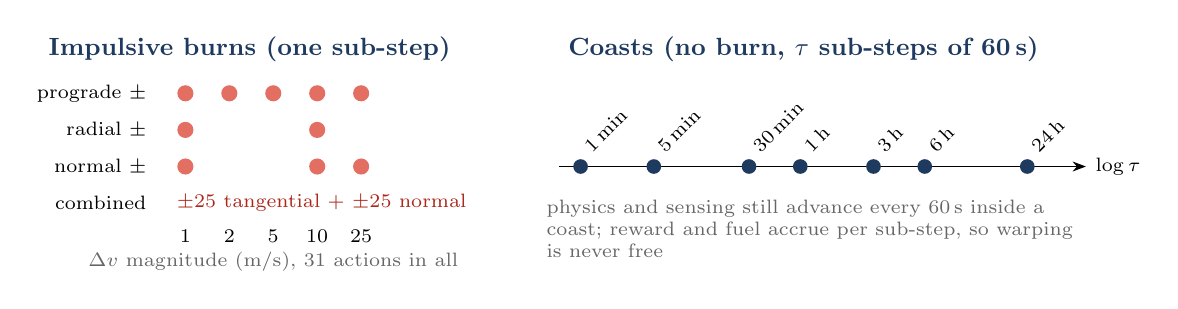
\begin{tikzpicture}[x=0.93cm,y=0.93cm]
  % burn panel
  \node[anchor=west,font=\small\bfseries,navy] at (0,3.1) {Impulsive burns (one sub-step)};
  \node[anchor=east,font=\scriptsize] at (1.6,2.5) {prograde $\pm$};
  \foreach \x in {2.0,2.6,3.2,3.8,4.4}{ \fill[accent!70] (\x,2.5) circle (0.11); }
  \node[anchor=east,font=\scriptsize] at (1.6,2.0) {radial $\pm$};
  \foreach \x in {2.0,3.8}{ \fill[accent!70] (\x,2.0) circle (0.11); }
  \node[anchor=east,font=\scriptsize] at (1.6,1.5) {normal $\pm$};
  \foreach \x in {2.0,3.8,4.4}{ \fill[accent!70] (\x,1.5) circle (0.11); }
  \node[anchor=east,font=\scriptsize] at (1.6,1.0) {combined};
  \node[font=\scriptsize,accent!80!black,anchor=west] at (1.75,1.0) {$\pm25$ tangential $+$ $\pm25$ normal};
  \foreach \x/\m in {2.0/1, 2.6/2, 3.2/5, 3.8/10, 4.4/25}{ \node[font=\scriptsize] at (\x,0.55) {\m}; }
  \node[font=\scriptsize,grey] at (3.2,0.2) {\dv\ magnitude (m/s), 31 actions in all};
  % coast panel
  \begin{scope}[xshift=6.6cm]
  \node[anchor=west,font=\small\bfseries,navy] at (0,3.1) {Coasts (no burn, $\tau$ sub-steps of 60\,s)};
  \draw[-{Stealth}] (0,1.5) -- (7.2,1.5) node[right,font=\scriptsize] {$\log\tau$};
  \foreach \x/\lab in {0.3/1\,min, 1.3/5\,min, 2.6/30\,min, 3.3/1\,h, 4.3/3\,h, 5.0/6\,h, 6.4/24\,h}{
    \fill[navy] (\x,1.5) circle (0.1);
    \node[font=\scriptsize,rotate=45,anchor=west] at (\x,1.65) {\lab};
  }
  \node[font=\scriptsize,grey,text width=7cm,align=left] at (3.6,0.65) {physics and sensing still advance every 60\,s inside a coast; reward and fuel accrue per sub-step, so warping is never free};
  \end{scope}
\end{tikzpicture}
\vspace{1mm}
\begin{itemize}\small
  \item A LEO phasing problem is thousands of minutes long; without coasts the credit-assignment horizon kills learning.
  \item With coasts the headline policy takes \key{24 decisions per episode}; the 24\,h coast is what lets J2 do a plane change for free.
\end{itemize}
\note{Semi-MDP is the precise term. Actions 0-15 is the legacy head (2-D), 20 the 3-D head, 31 with the day-warp. If asked about action masking: none; the policy learns which actions are available by consequence.}
\end{frame}

% =====================================================================
\begin{frame}{Policy and training: a small recurrent network trained with PPO}
\begin{columns}[T]
\begin{column}{0.5\textwidth}
\centering
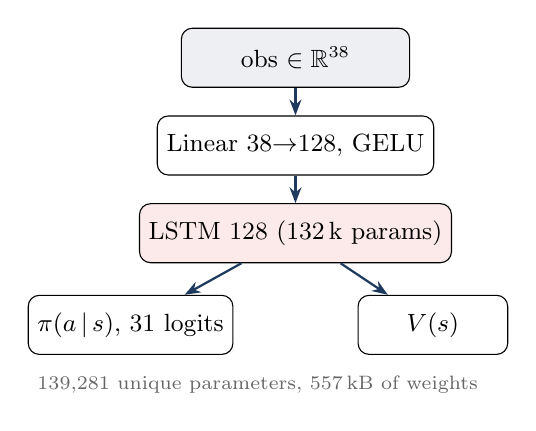
\begin{tikzpicture}[
  nb/.style={draw,rounded corners,minimum width=2.9cm,minimum height=0.75cm,font=\small,fill=white},
  arr/.style={-{Stealth[length=2mm]},thick,navy}]
  \node[nb,fill=navy!8] (o) {obs $\in\mathbb R^{\nObs}$};
  \node[nb,below=0.35cm of o] (e) {Linear \nObs$\to$128, GELU};
  \node[nb,below=0.35cm of e,fill=accent!10] (l) {LSTM 128 (132\,k params)};
  \node[nb,below left=0.4cm and -1.2cm of l,minimum width=1.9cm] (a) {$\pi(a\,|\,s)$, 31 logits};
  \node[nb,below right=0.4cm and -1.2cm of l,minimum width=1.9cm] (v) {$V(s)$};
  \draw[arr] (o)--(e); \draw[arr] (e)--(l); \draw[arr] (l)--(a); \draw[arr] (l)--(v);
  \node[font=\scriptsize,grey,below=0.15cm of a.south west,anchor=north west] {\nParams\ unique parameters, 557\,kB of weights};
\end{tikzpicture}
\end{column}
\begin{column}{0.5\textwidth}\small
\textbf{Why an LSTM} \; the estimate's history carries information the instantaneous state does not (is the filter converging? did that burn do what I expected?)\\[1.5mm]
\textbf{PPO} \; \nEnvs\ envs, $\gamma=0.995$, clipped surrogate $\pm0.2$, GAE $\lambda=0.9$, entropy 0.01, Muon optimizer, 50\,M steps per curriculum rung (about 2\,h each)\\[1.5mm]
\textbf{Reward} \; $+1$ success, $-1$ failure, dense potential-difference shaping on the \emph{mean-longitude} gap and element match, clamped to $[-1,1]$\\[1.5mm]
\textbf{Curriculum} \; one variable per rung, warm-started: circular at the full $\pm180^\circ$ gap $\to$ eccentric $\to$ wide envelope $\to$ 3-D $\to$ estimate in the loop $\to$ the seven-skill mixture. Fresh training at the hard endpoint flat-lines.
\end{column}
\end{columns}
\note{If asked why not a bigger net: 140k parameters is enough and it has to run on a flight processor. If asked about shaping being a crutch: it is potential-based with gamma_shape = 1, so it does not change the optimal policy; the ablation without it peaks at 3.6 percent. If asked about the clamp: it is in the trainer; it caps the per-step gradient from rare terminal events.}
\end{frame}

% =====================================================================
\begin{frame}{Headline, 2-D: every held-out episode rendezvous, on every training seed}
\centering
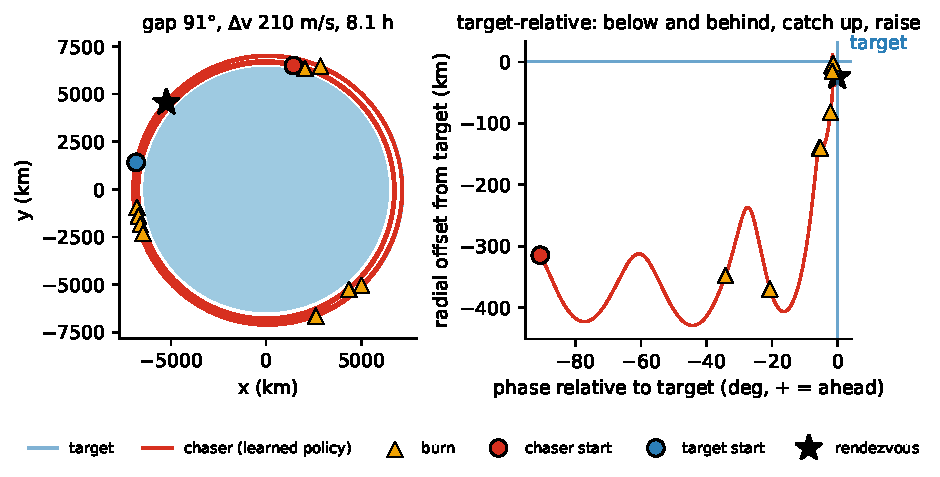
\includegraphics[width=0.6\textwidth]{traj_rendezvous.pdf}
\vspace{-1mm}
\begin{columns}[T]
\begin{column}{0.62\textwidth}\footnotesize
\begin{itemize}
  \item \key{200/200} held-out episodes (eval seed 123) for \key{\headlineSeeds}, including the seed that had flat-lined at 0\,\% before the dynamics fix.
  \item Re-run for this deck on a fresh evaluation seed: 200/200.
  \item Wide envelope (300--8,000\,km, $e\le0.30$): 4 seeds, 800/800; 3,199/3,200 over the whole four-rung ladder.
\end{itemize}
\end{column}
\begin{column}{0.36\textwidth}\scriptsize\textcolor{grey}{
Shown: a $91^\circ$ gap closed in 8.1\,h with 210\,m/s; low and behind, catch up, then raise. \texttt{models/t3/seed42\_L2\_headline.pt}.}
\end{column}
\end{columns}
\note{This is the "it works" slide. The phasing picture is the physics: lower orbit = shorter period = catch up. Point at the burn triangles: early retro to drop, late prograde to raise.}
\end{frame}

% =====================================================================
\begin{frame}{How good is it? Audit against an optimal-control comparator}
\begin{columns}[T]
\begin{column}{0.56\textwidth}
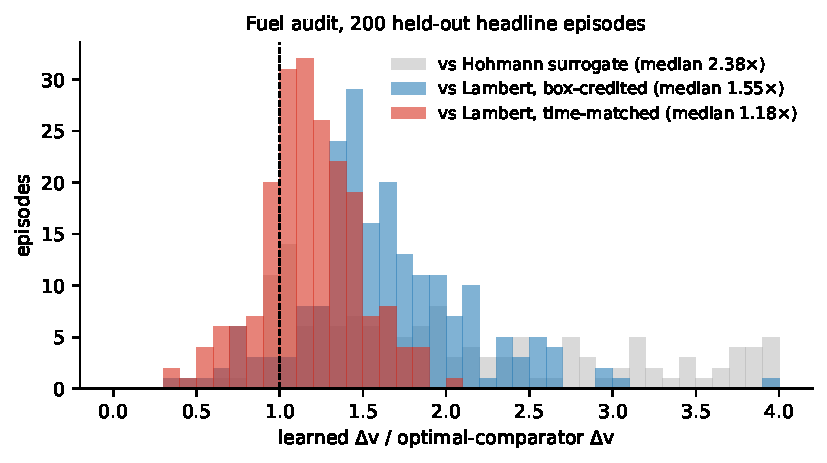
\includegraphics[width=0.96\textwidth]{dv_ratio.pdf}
\end{column}
\begin{column}{0.44\textwidth}\footnotesize
\textbf{Comparator} \; a Lambert solver (Izzo--Lancaster universal variables, multi-rev, both branches) searched over departure wait $\times$ time of flight, with perfect information.\\[1.5mm]
\textbf{Fair denominator} \; same episode, same time budget: median \key{\lambertRatio} the optimum.\\[1mm]
\textbf{Credited to the box} \; \boxRatio.\\[1mm]
\textbf{Hohmann surrogate} \; \hohmannRatio, but it ignores phasing and the velocity match, so it was retired as the headline.\\[1.5mm]
{\scriptsize\textcolor{grey}{200 held-out episodes, \texttt{web\_data/results/fuel\_audit.csv}. Ratios below 1 are possible because arrival is credited inside a box, not at an exact state.}}
\end{column}
\end{columns}
\note{Why Lambert instead of Hohmann: Hohmann is a circular-to-circular transfer with no phasing; the task is phasing. Why the sin(180) singularity matters: the standard universal-variable form collapses at a 180-degree transfer, so I used the Lancaster-Blanchard / Izzo form. The porkchop is in the appendix.}
\end{frame}

% =====================================================================
\begin{frame}{Bearings-only navigation: the policy flies on an angles-only estimate}
\begin{columns}[T]
\begin{column}{0.5\textwidth}
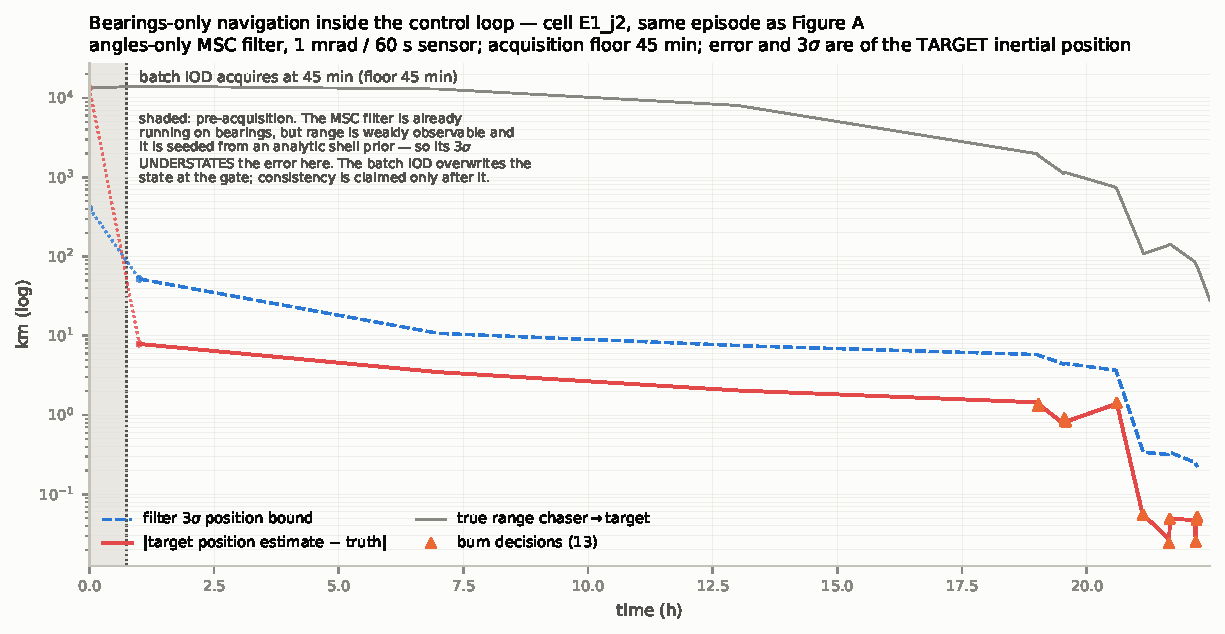
\includegraphics[width=\textwidth]{nav3d_estimate.pdf}\\
{\scriptsize\textcolor{grey}{3-D, cell E1\_j2, same episode as the generalist slide. Shaded: blind, angles accumulating. After acquisition the estimate error (red) collapses as range closes; dashed is the filter's own $3\sigma$ claim.}}
\end{column}
\begin{column}{0.5\textwidth}\small
\textbf{Sensor} \; line-of-sight angles only, 1\,mrad noise, one per 60\,s sub-step; range is never measured\\[1mm]
\textbf{Acquire} \; batch initial-orbit determination: range-hypothesis lattice along the first ray, Levenberg-damped Gauss--Newton, accepted on a $\chi^2$ test and a runner-up margin\\[1mm]
\textbf{Track} \; recursive filter in log-spherical coordinates seeded by the batch solution; calibration checked per channel (a range/bearing EKF with NEES/NIS is in A4)\\[1mm]
\textbf{Result} \; a policy trained on truth and handed the estimate: \key{51\,\%}. Retrained with the filter in the loop: \key{97\,\%} (2-D tight box, one seed); \key{46\,\%$\to$98\,\%} in 3-D across three seeds.\\[1mm]
{\scriptsize\textcolor{grey}{It did not learn to \emph{probe} (measured null); it learned to wait for acquisition and burn nothing while blind (median \dv\ before acquisition 75$\to$0\,m/s).}}
\end{column}
\end{columns}
\note{Huber bridge: an EO payload on orbit produces exactly this measurement. The key engineering finding: the estimator is not the bottleneck at realistic noise; the policy has to be trained on the estimate, not on truth. Noise sweep and NEES plots are in the appendix.}
\end{frame}

% =====================================================================
\begin{frame}{The generalist: one policy, seven rendezvous skills, 3-D with J2}
\centering
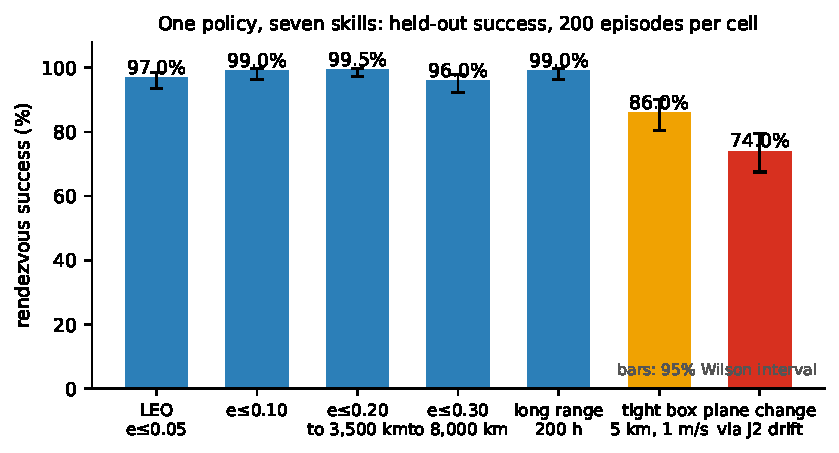
\includegraphics[width=0.8\textwidth,height=0.6\textheight,keepaspectratio]{generalist_cells.pdf}
\begin{flushleft}
\vspace{-1mm}{\scriptsize\textcolor{grey}{All cells: 3-D, J2, bearings-only navigation, fuel budget sampled per episode, 200 held-out episodes each, one training seed. Tight box reaches 92.5\,\% at its training fuel floor. Single-skill specialists average 6--42\,\% off their home cell, which is why one policy was worth building. Cell definitions in A5.}}
\end{flushleft}
\note{This is the centrepiece. Five skills at 96-99.5, tight box 86 (92.5 at training floor), plane change 74. The plane-change skill is the only one where the policy exploits J2: it dips low, waits for the node to drift, and uses day-long coasts; a 3-degree plane change by burning would exceed the whole tank.}
\end{frame}

% =====================================================================
\begin{frame}{The generalist flying: 3-D, J2, bearings-only, one of the 200 held-out episodes}
\centering
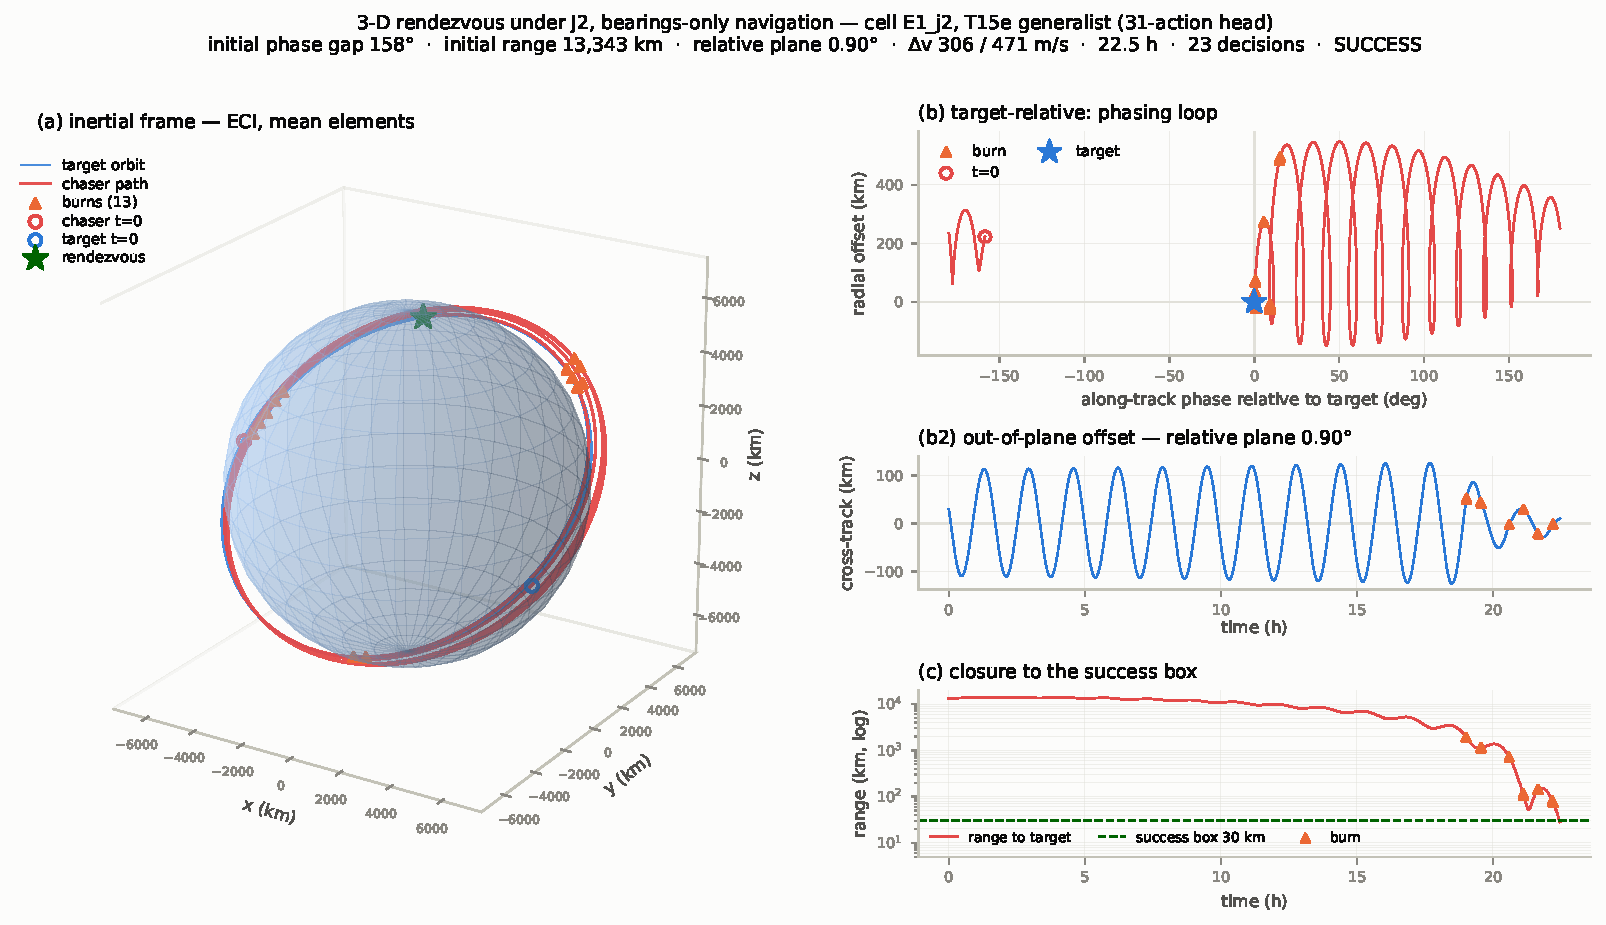
\includegraphics[width=0.92\textwidth,height=0.74\textheight,keepaspectratio]{traj3d_rendezvous.pdf}
\\[-1mm]{\scriptsize\textcolor{grey}{Cell E1\_j2, T15e checkpoint. A $158^\circ$ gap and a $0.9^\circ$ plane difference closed in 22.5\,h with 306\,m/s of 471 and 23 decisions, flying on the filter's estimate. Panel (b) is the phasing loop seen from the target; (b2) the cross-track oscillation the plane burns null at the end; (c) the closure.}}
\note{Point at (b): the chaser parks above the target so the target catches up, then descends. Panel (b2): out-of-plane is left alone until the end, then nulled with three normal burns. Everything here is what an EO sensor on the chaser would see turned into a decision.}
\end{frame}

% =====================================================================
\begin{frame}{How it got there: measuring interference, then fixing it}
\begin{columns}[T]
\begin{column}{0.5\textwidth}
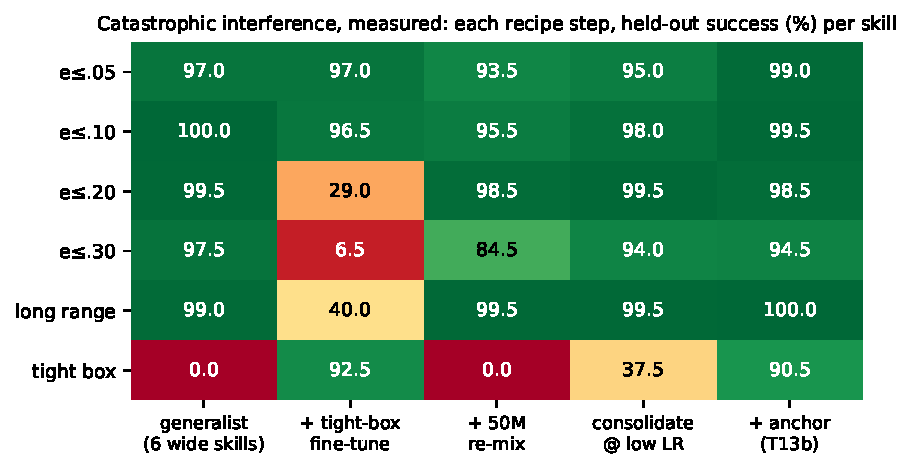
\includegraphics[width=\textwidth]{seesaw.pdf}
\end{column}
\begin{column}{0.5\textwidth}
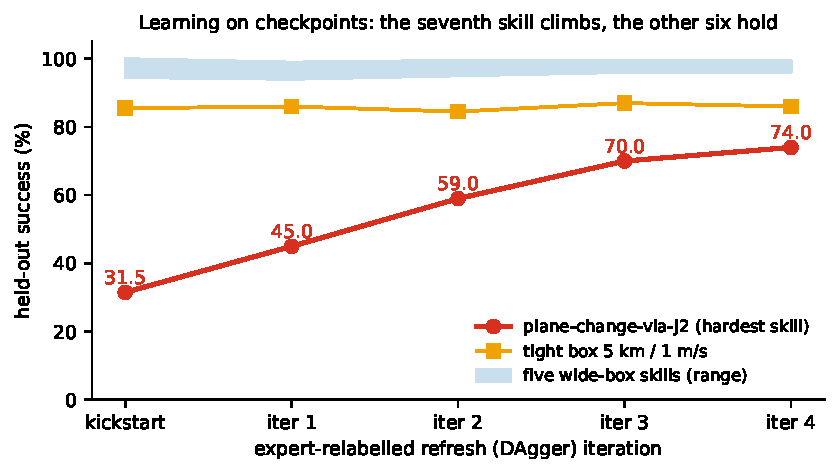
\includegraphics[width=\textwidth]{dagger_curve.pdf}
\end{column}
\end{columns}
\small
\begin{itemize}
  \item Fine-tuning for the tight box destroyed three other skills; re-mixing restored them and lost the tight box. A low-learning-rate consolidation with an \key{anchor} (replay of the specialist's own trajectories) held all six.
  \item The seventh skill came from four rounds of \key{expert-relabelled refresh} (DAgger against a scripted GNC expert), with a stopping rule fixed before the numbers existed. Reproduced at a second seed (33.5\,\% start, $+14$ first step).
\end{itemize}
\note{If asked "where is your training curve": the headline recovery runs never logged a curve; what I trust is this learning-on-checkpoints series, 31.5 to 74, every point a 200-episode held-out eval. The seesaw is the honest picture of catastrophic interference.}
\end{frame}

% =====================================================================
\begin{frame}{Verification is the story: what I caught, and what is still open}
\begin{columns}[T]
\begin{column}{0.5\textwidth}\footnotesize
\textbf{Caught}
\begin{itemize}
  \item A swapped half-angle factor in the true-to-mean anomaly conversion let every burn teleport phase (median $25^\circ$ per episode). The old headline fell from 97.5\,\% to 13\,\% under correct dynamics; every number here is post-fix.
  \item A reward leak that made coast-only policies look capable at high altitude (null test: a zero policy reproduced it).
  \item A red team on the filter: a coordinate-chart swap was a measured null; an unscented filter restored calibration without it.
  \item A numbered ledger of metric-versus-implementation bugs, each with a before/after number.
\end{itemize}
\end{column}
\begin{column}{0.5\textwidth}\footnotesize
\textbf{Still open}
\begin{itemize}
  \item Generalist and the 2-D 51$\to$97 arm are single-seed; the 2-D headline, wide envelope, 3-D nav and J2 rungs are multi-seed.
  \item Fuel is \lambertRatio\ the Lambert optimum, not 1.0; the action grid is coarse.
  \item Chaser navigation is assumed perfect; no eclipses, dropouts, or sensor bias.
  \item Arrival is certified, not station-keeping; two-body plus secular J2 only.
\end{itemize}
\textbf{Next}
\begin{itemize}
  \item Relative-state filter with chaser error; measurement gating; multi-seed generalist.
  \item A matched MPC comparator; a maneuvering target.
\end{itemize}
\end{column}
\end{columns}
\note{Close on this. The posture: I would rather show you the bug I found than a number I cannot defend. Then open for questions and jump to the appendix as needed.}
\end{frame}

% =====================================================================
\appendix
\begin{frame}[plain]
  \centering{\Large\textcolor{navy}{\textbf{Appendix}}}\\[2mm]
  \small observation vector \;$\cdot$\; action table \;$\cdot$\; Kepler and Lambert \;$\cdot$\; J2 \;$\cdot$\; filter consistency \;$\cdot$\; noise sweep \;$\cdot$\; the seven cells \;$\cdot$\; embedded port \;$\cdot$\; dynamics bug \;$\cdot$\; red team
\end{frame}

\begin{frame}{A1 \; Observation vector (\nObs\ floats, all roughly in $[-1,1]$)}
\tiny
\begin{tabular}{@{}lll@{}}
\toprule
slots & value & why\\
\midrule
0--1 & chaser altitude / scale, $e$ & size and shape\\
2--3 & $\sin\theta,\cos\theta$ & position on orbit, no wrap\\
4--5 & $v_r/v_{circ},\ v_t/v_{circ}$ & radial and tangential speed\\
6 & fuel fraction & budget remaining\\
7--8 & target altitude, $e$ (estimated) & target size and shape\\
9--12 & $\sin,\cos\,\omega$ for both & apse orientations\\
13--14 & $\sin,\cos\,\Delta\lambda$ (mean longitude gap) & the phase gap, gauge-corrected in 3-D\\
15 & (cap $-$ step)/cap & episode clock\\
16 & $\cos(\omega_s-\omega_t)$ & apsidal alignment\\
17--20 & nearest body: distance, bearing, closing rate, keep-out & Earth\\
21--25 & relative-inclination vector in chaser axes; $\Delta\mathbf e\cdot\hat h_t$; cross-track offset and rate & 3-D block\\
26--28 & $\dv_{plane},\ \dv_{remaining}$, feasibility margin & fuel ledger\\
29--30 & $\cos i_s,\ \cos i_t$ & J2 only\\
33--36 & LVLH radial / along-track offset; relative velocity with rotating-frame correction & rectilinear relative state\\
37 & target mean motion & \\
\bottomrule
\end{tabular}
\\[1mm]\textcolor{grey}{All target quantities are the filter's estimate in bearings-only mode. The policy is not given the covariance (tested: a $\sigma$ channel added nothing).}
\end{frame}

\begin{frame}{A2 \; Why a lower orbit catches up, and what J2 gives for free}
\begin{columns}[T]
\begin{column}{0.5\textwidth}\footnotesize
\textbf{Phasing} \; $T = 2\pi\sqrt{a^3/\mu}$, so a chaser 100\,km below a LEO target gains about $4^\circ$ of phase per orbit. Drop, wait $N$ orbits, raise: the policy's catch-up pattern is the textbook phasing manoeuvre, discovered from reward alone.\\[2mm]
\textbf{Plane change by burning} \; $\dv = 2v\sin(\Delta i/2)$; at 7.5\,km/s a $3^\circ$ change costs $\sim$390\,m/s, most of the tank.\\[2mm]
\textbf{Plane change by J2} \; $\dot\Omega = -\tfrac32 J_2 n (R_E/p)^2 \cos i$ depends on $a$ and $i$, so two orbits at different altitudes drift apart in $\Omega$ at a controllable rate. The seventh skill dips low, coasts a day at a time, and lets differential nodal precession close the plane gap (about half the alignment bought this way in the specialist).
\end{column}
\begin{column}{0.5\textwidth}
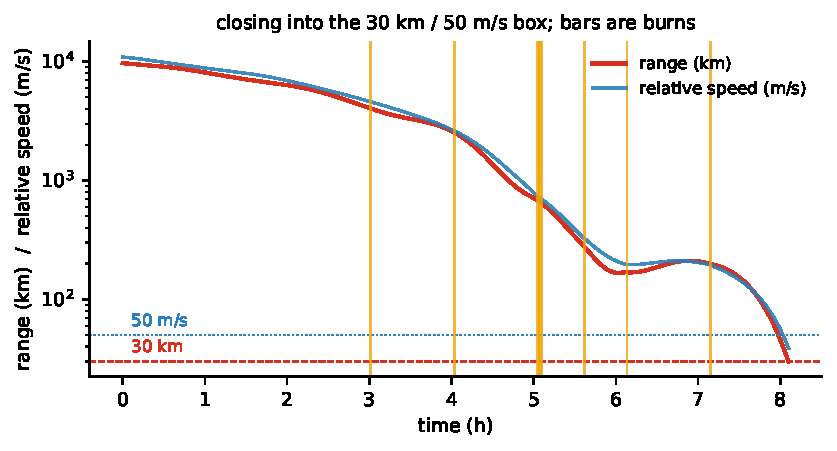
\includegraphics[width=0.85\textwidth]{traj_closing.pdf}
\end{column}
\end{columns}
\end{frame}

\begin{frame}{A3 \; Lambert comparator: the search the policy is being graded against}
\begin{columns}[T]
\begin{column}{0.55\textwidth}
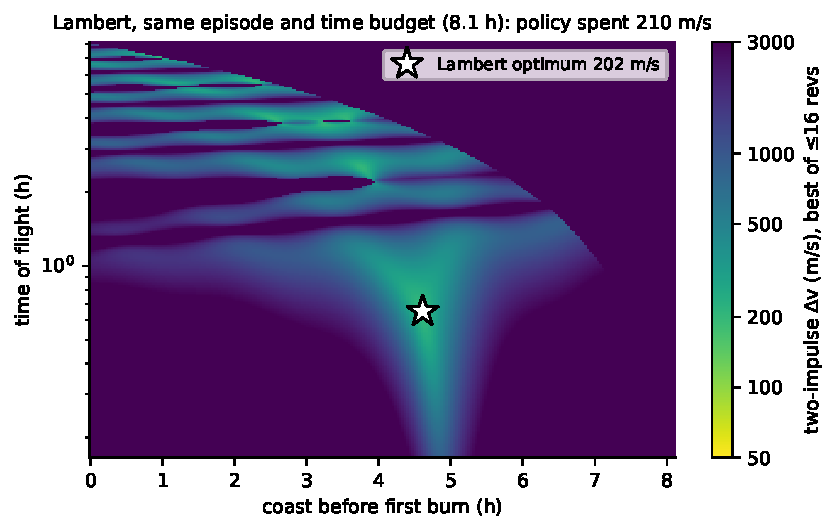
\includegraphics[width=\textwidth]{lambert_porkchop.pdf}
\end{column}
\begin{column}{0.45\textwidth}\small
Given $\mathbf r_1,\mathbf r_2$ and a flight time, find the conic that connects them: Lambert's problem.\\[1mm]
Standard universal-variable form has $A=\sin\Delta\theta\sqrt{r_1 r_2/(1-\cos\Delta\theta)}$, which vanishes at a $180^\circ$ transfer, exactly the hard phase gap. So the solver uses the Lancaster--Blanchard / Izzo parameterisation in $\lambda$ and $x$, with closed-form derivatives of the time-of-flight for a Householder iteration, and multi-revolution branches.\\[1mm]
The comparator grids departure wait $\times$ time of flight (log-spaced), takes the minimum over revolution counts and branches, then refines around the best cell four times.\\[1mm]
{\scriptsize\textcolor{grey}{This episode: optimum 202\,m/s under the policy's own 8.1\,h budget; the policy spent 210\,m/s.}}
\end{column}
\end{columns}
\end{frame}

\begin{frame}{A4 \; Range/bearing EKF: consistency and sensor-noise robustness (2-D)}
\begin{columns}[T]
\begin{column}{0.5\textwidth}
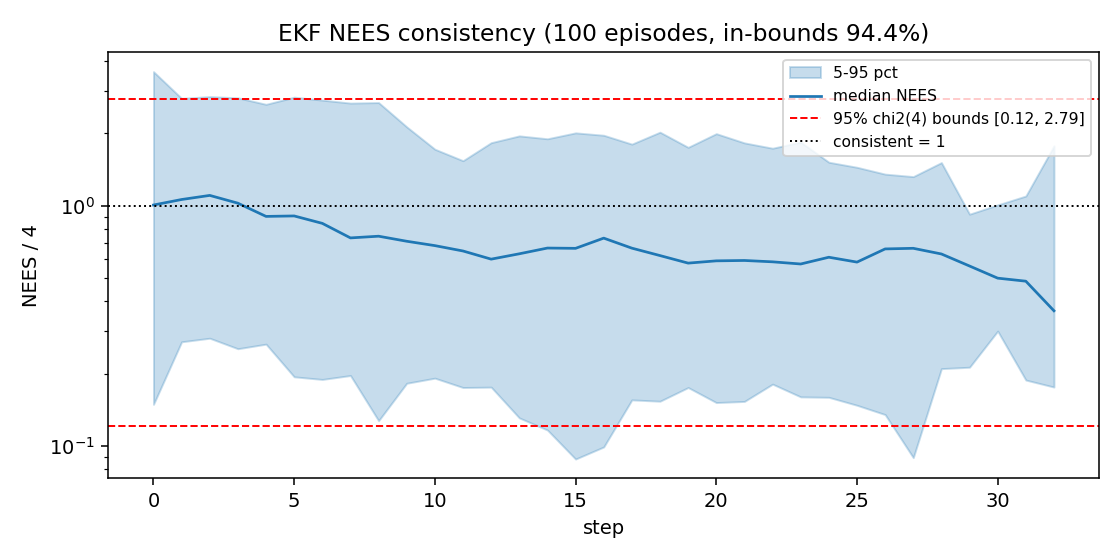
\includegraphics[width=0.84\textwidth]{nees.png}\\
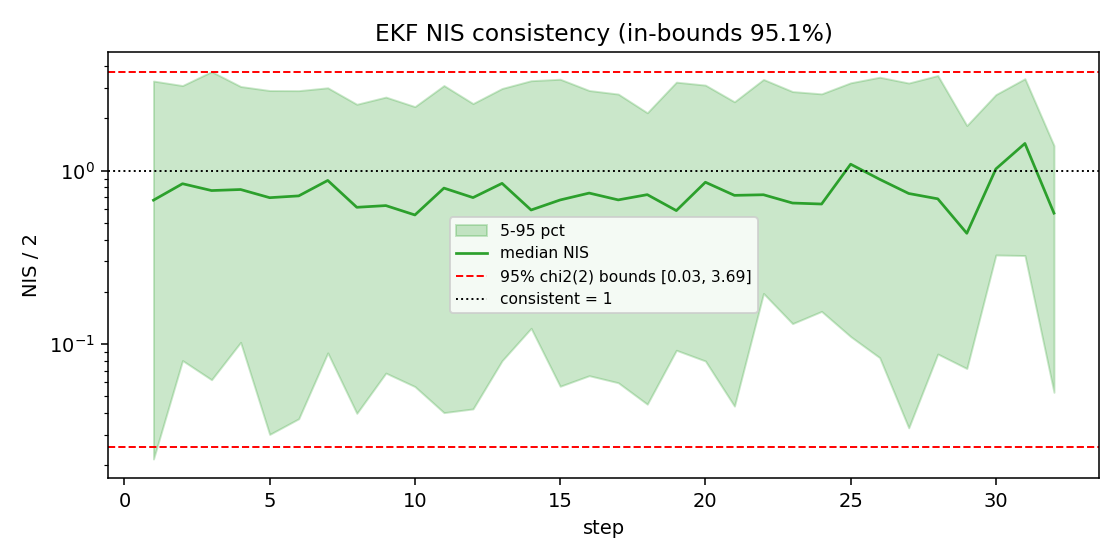
\includegraphics[width=0.84\textwidth]{nis.png}
\end{column}
\begin{column}{0.5\textwidth}
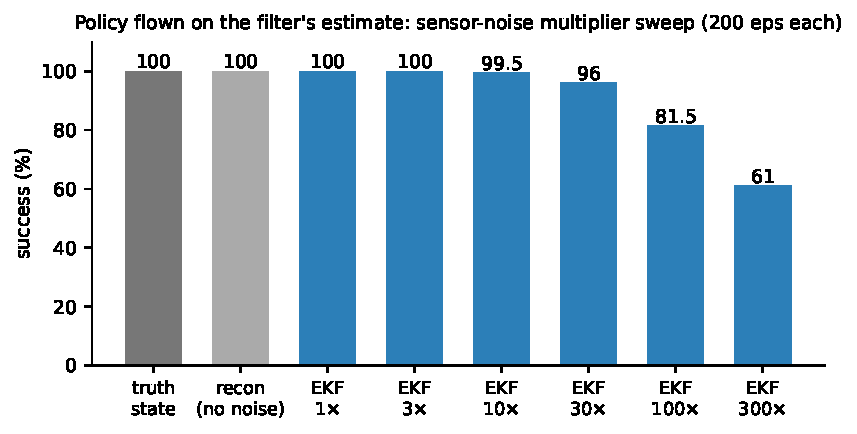
\includegraphics[width=\textwidth]{noise_sweep.pdf}
\footnotesize
NEES $=\tilde{\mathbf x}^\top P^{-1}\tilde{\mathbf x}$ tests the state covariance; NIS $=\boldsymbol\nu^\top S^{-1}\boldsymbol\nu$ tests the innovation covariance. Both reported as the fraction of steps inside the 95\,\% $\chi^2$ band.\\[1mm]
{\scriptsize\textcolor{grey}{2-D range/bearing EKF ($\sigma_\rho$ 50\,m, $\sigma_\beta$ 1\,mrad) on the headline policy; flat to 10$\times$ noise because converged error (tens of metres) is far inside the 30\,km box; beyond 30$\times$ the limit is filter divergence.}}
\end{column}
\end{columns}
\end{frame}

\begin{frame}{A5 \; The seven cells of the generalist mixture}
\scriptsize
\begin{tabular}{@{}llllllr@{}}
\toprule
cell & $a$ range (km altitude) & $e_{max}$ & box & clock (sub-steps) & weight & success\\
\midrule
E0\_j2 & 300--800 & 0.05 & \boxR\,/\,\boxV & 3,000 & 0.15 & 97.0\,\%\\
E1\_j2 & 300--1,500 & 0.10 & \boxR\,/\,\boxV & 3,000 & 0.15 & 99.0\,\%\\
E2\_j2 & 300--3,500 & 0.20 & \boxR\,/\,\boxV & 4,500 & 0.15 & 99.5\,\%\\
E3\_j2 & 300--8,000 & 0.30 & \boxR\,/\,\boxV & 6,000 & 0.15 & 96.0\,\%\\
LONGRANGE & 300--3,500 & 0.12 & \boxR\,/\,\boxV & 12,000 & 0.10 & 99.0\,\%\\
TIGHT\_5k1 & 300--800 & 0.05 & \tightR\,/\,\tightV & 3,000 & 0.10 & 86.0\,\%$^\dagger$\\
W1\_driftwait & 300--800 & 0.05 & \boxR\,/\,\boxV & 22,000 & 0.20 & 74.0\,\%\\
\bottomrule
\end{tabular}
\\[2mm]
$^\dagger$92.5\,\% at the training fuel floor. LONGRANGE is a $\sim$500\,km transfer under a 12,000-sub-step clock. All cells: 3-D, J2 on, bearings-only navigation with real batch acquisition, Discrete(31) head, fuel budget sampled per episode (353--656\,m/s) so the policy is fuel-aware. Held-out evaluation seed 123, 200 episodes per cell, greedy action selection, LSTM state zeroed per episode.\\[1mm]
{\scriptsize\textcolor{grey}{Source: \texttt{pufferlib/ocean/orbital/t11\_cells.py}, \texttt{web\_data/results/t15e\_dagger/fin\_*.json}, \texttt{T11\_GENERALIST.md}.}}
\end{frame}

\begin{frame}{A6 \; Embedded C port: the policy as flight software}
\begin{columns}[T]
\begin{column}{0.5\textwidth}
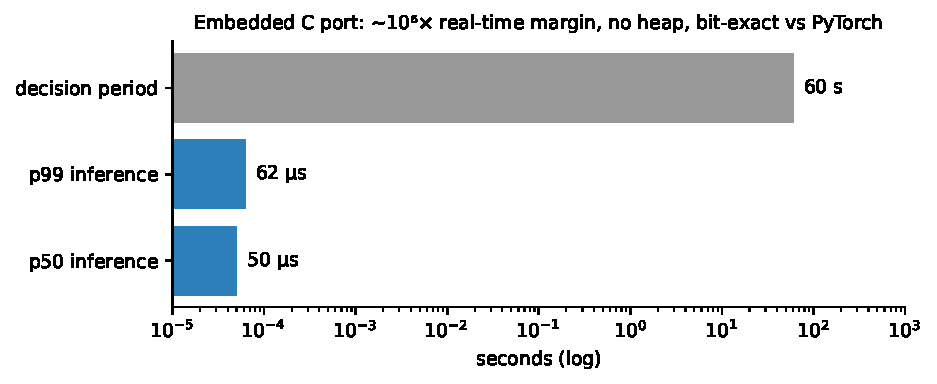
\includegraphics[width=0.7\textwidth]{cport_timing.pdf}
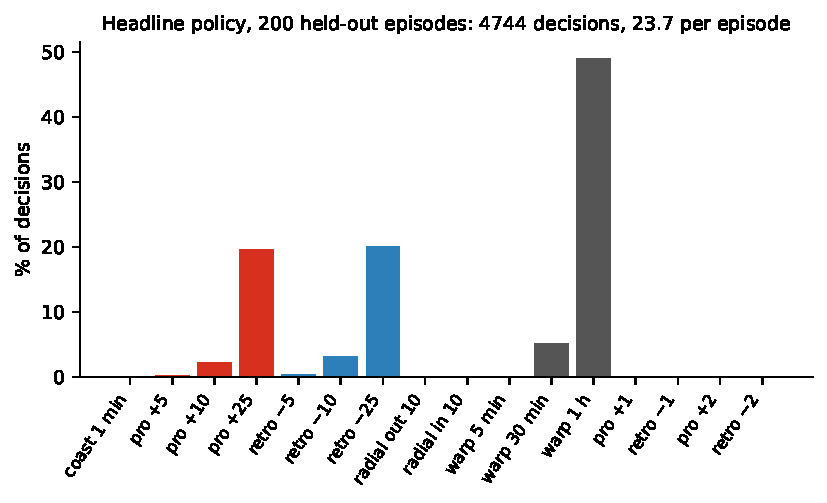
\includegraphics[width=0.7\textwidth]{action_hist.pdf}
\end{column}
\begin{column}{0.5\textwidth}\footnotesize
\begin{itemize}
  \item No heap: weights are 557\,kB of read-only data; recurrent state 1,032 bytes owned by the caller; worst-case stack 3,840 bytes.
  \item Bounded execution: 138,112 multiply-accumulates per call regardless of input.
  \item Fail-safe commit: NaN from a bad sensor is rejected, LSTM memory untouched, loop coasts that frame.
  \item Deterministic, reentrant; ASan and UBSan clean.
  \item Parity: 100\,\% action agreement over 7,048 observation vectors; 200/200 closed-loop episodes with an identical action stream to PyTorch.
  \item p99 \pNinetyNine\ on an M3 Max (a desktop timing, not a WCET) against a 60\,s decision period.
\end{itemize}
\end{column}
\end{columns}
\end{frame}

\begin{frame}{A7 \; The dynamics bug, and why every number here is post-fix}
\small
\begin{columns}[T]
\begin{column}{0.5\textwidth}
\textbf{What} \; the true-anomaly $\to$ mean-anomaly conversion, called only after a burn, had its $\sqrt{1\pm e}$ factors swapped. Each burn off an apse silently moved the chaser along-track (up to 700\,km at $e=0.05$); a median $25^\circ$ of free phasing per episode. Burns at apsides were unaffected, so every unit test passed.\\[2mm]
\textbf{How it was found} \; twice on the same day: by formula inspection while porting the dynamics into the navigation filter, and by the Lambert audit, where 15\,\% of episodes beat half the time-matched two-impulse optimum. A diagnostic then showed an $86.5^\circ$ true-anomaly jump for a 25\,m/s burn against a 1\,km displacement.\\[2mm]
\textbf{Cost} \; the then-canonical checkpoint went from 97.5\,\% to 13\,\% under corrected dynamics. All pre-fix checkpoints and numbers were retired.
\end{column}
\begin{column}{0.5\textwidth}
\textbf{Recovery recipe} (each piece ablated)
\begin{itemize}
  \item potential shaping on the \emph{mean-longitude} gap with $\gamma_{shape}=1$
  \item physical-gap initialisation and a fixed phase observation
  \item an episode-clock observation; cap reward 0 not $-10$
  \item scripted GNC expert as a reference: 99.2\,\%
\end{itemize}
\textbf{Lesson} \; the comparator caught what the success metric could not. Audits against physics are part of the training loop, not a report at the end.
\end{column}
\end{columns}
\end{frame}

\begin{frame}{A8 \; Red team on the navigation filter}
\small
\begin{itemize}
  \item \textbf{Hypothesis} \; the EKF's coordinate chart (Cartesian) was causing the acquisition-stage fragility; a modified-spherical-coordinates chart should fix it.
  \item \textbf{Test} \; chart swapped in the closed loop, 2-D and 3-D, same seeds, same episodes.
  \item \textbf{Result} \; a measured null: 2-D $-1/0/0/-4/+1$ per 200 across five arms; 3-D $-0.17$\,pp with a $[-1.2,+0.8]$ interval. Production filters reproduced the prototype's fragility; an unscented filter recovered calibration without a chart change.
  \item \textbf{What actually fixed acquisition} \; batch initial-orbit determination before handing off to the filter (never-acquire episodes 44/200 $\to$ 0/200).
  \item \textbf{Why report it} \; five claims in my own interview notes were contradicted by this test. The document was corrected.
\end{itemize}
\vspace{2mm}
{\scriptsize\textcolor{grey}{\texttt{reports/msc\_REDTEAM.md} \S9.}}
\end{frame}

\begin{frame}{A9 \; If asked}
\scriptsize
\begin{description}
  \item[Why RL at all, when Lambert exists?] Lambert needs perfect state and gives an open-loop plan; the policy is closed-loop on an estimate, handles a budget, and the same network covers seven regimes. Lambert is my grader, not my competitor.
  \item[Why discrete actions?] PPO is stable with them; a continuous Box(2) head collapsed in early trials. The grid costs fuel (1.14--1.18$\times$ the time-matched optimum across two evaluation sets); finer grades are the obvious next step.
  \item[Why not MPC?] It would be the right production baseline. The project's question was whether a learned policy can close the loop on estimated state across regimes; MPC with the same filter is the comparison I would run next.
  \item[Is 200 episodes enough?] For a 97\,\% point the Wilson 95\,\% interval is about $\pm2.5$\,pp; for 0/200 the two-sided Clopper--Pearson lower bound is 98.2\,\%. I report intervals, and I do not say 100\,\% means zero.
  \item[Single seed?] The generalist, yes. The 2-D headline (5 seeds), wide envelope (4), 3-D nav rungs (3), J2 tight box (3) are multi-seed.
  \item[Why does the policy coast 24 h?] Because J2 node regression closes an inclination gap for free; burning it would exceed the tank. It learned that.
  \item[What would you do differently?] Audit against physics from day one; log learning curves on every run; design the observation with the filter in mind from the start.
\end{description}
\end{frame}

\end{document}
